\documentclass[FM,DP]{tulthesis}
% tento dokument používá balíky specifické pro XeLaTeX a lze jej přeložit
% jen XeLaTeXem, nemáte-li instalována použitá (komerční) písma, změňte
% nebo vymažte příkazy \set...font na následujících řádcích

\newcommand{\verze}{1.10}

\usepackage{polyglossia}
\setdefaultlanguage{czech}
\usepackage{xevlna}
\usepackage{graphicx}
\usepackage{float}
\usepackage{makeidx}
\makeindex

% fonty
\usepackage{fontspec}
\usepackage{xunicode}
\usepackage{xltxtra}

% příkazy specifické pro tento dokument
\newcommand{\argument}[1]{{\ttfamily\color{\tulcolor}#1}}
\newcommand{\argumentindex}[1]{\argument{#1}\index{#1}}
\newcommand{\prostredi}[1]{\argumentindex{#1}}
\newcommand{\prikazneindex}[1]{\argument{\textbackslash #1}}
\newcommand{\prikaz}[1]{\prikazneindex{#1}\index{#1@\textbackslash #1}}
\newenvironment{myquote}{\begin{list}{}{\setlength\leftmargin\parindent}\item[]}{\end{list}}
\newenvironment{listing}{\begin{myquote}\color{\tulcolor}}{\end{myquote}}
\sloppy
\graphicspath{ {./images/} }

% deklarace pro titulní stránku
\TULtitle{Software pro správu projektu}

% pro bakalářské, diplomové a disertační práce
\TULyear{2022}
\TULprogramme{B0613A140005}{Informační technologie}{Information technology}
\TULauthor{Kevin Daněk}
\TULsupervisor{doc. Ing. Jiřina Královcová, Ph.D.}
\TULthesisType{Semestrální práce}{Semestral work}

\begin{document}

\ThesisStart{male}
%\ThesisStart{zadani-a-prohlaseni.pdf}

\begin{abstractCZ}
Cílem semestrální práce bylo navrhnout a realizovat informační systém v jazyce Java.
\end{abstractCZ}

\begin{keywordsCZ}
Java
\end{keywordsCZ}

\vspace{2cm}

\begin{abstractEN}
This report describes the \texttt{tulthesis} package for Technical university of
Liberec thesis typesetting using the \LaTeX\ typographic system.
\end{abstractEN}

\begin{keywordsEN}
\LaTeX, class, TUL
\end{keywordsEN}

\tableofcontents

\chapter{Zadání}
Cílem práce je vytvořit program, který bude realizovat správu vývoje softwaru pomocí metody Kanban. Metodou Kanban rozumíme rozdělení práce na menšéíé úkoly, které se postupně přesouvají vývojem z různých sloupců až do stavu, kdy jsou označeny za hotovy.

\begin{figure}[H]
	\centering
	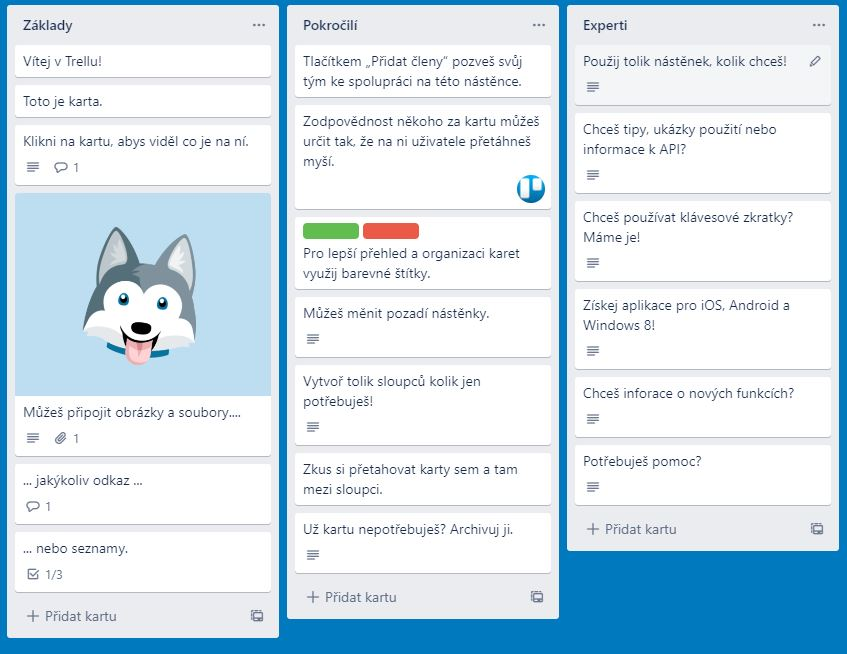
\includegraphics[width=0.75\textwidth]{trello-example}
	\caption{Ukázka vizuální reprezentace metody Kanban (Ze služby Trello)}
\end{figure}

Program by měl být schopný
\begin{itemize}
	\item \textbf{vytvořit a spravovat} vícero nástěnek
	\item \textbf{přidávat a spravovat sloupce} v nástěnkách
	\item \textbf{přidávat a spravovat úkoly} ve sloupcích
	\item \textbf{přidávat a přidělovat} zaměstnance
\end{itemize}

\chapter{Specifikace implementace}

\section{Formát dat}
Program ukládá svá data do souborů formátu JSON. Každý klíč (až na vyhrazený klíč \texttt{class}) odpovídá atributu objektu (instance třídy), kde hodnota představuje okamžitou hodnotu v době uložení na disk.

\section{Závislost tříd}
Architektura programu stojí na zjednodušeném MVC modelu, kde \textit{model} představují entity balíku \texttt{trello}, \textit{controller} třídy balíku \texttt{stores} a \textit{view} balík \texttt{ui}. Níže na obrázku lze vidět, jak se uživatel může pohybovat mezi pohledy. Plná čára značí krok, přerušovaná závislost, resp. dědičnost.

\begin{figure}[H]
	\centering
	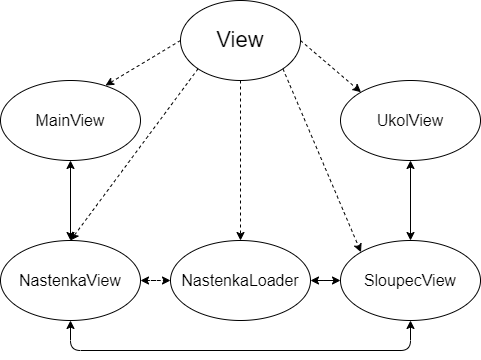
\includegraphics[width=0.75\textwidth]{ui}
	\caption{Závislosti a cesty mezi jednotlivými pohledy uživatelského rozhraní}
\end{figure}


\section{Kompetence tříd}
\subsection{Podbalík \texttt{trello}}
Třídy balíku \texttt{trello} reprezentují jednotlivé entity programu a slouží jako nositelé dat.

\subsection{Podbalík \texttt{stores}}
Balík \texttt{stores} slouží pro třídy, které aplikace používá pro ukládání dat do paměti a pro jednotný přístup k těmto datům. Tyto třídy jsou \texttt{singletony}, které uchovávají instance jednotlivých entit.

\subsubsection{Třída \texttt{NastenkaStore}}
Třída \texttt{NastenkaStore} je \texttt{singletonem}, který uchovává a poskytuje přístup k instanci třídy \texttt{Nastenka}. Umožňuje načíst, uložit a vypsat aktuální instanci ze souborového systému.

\subsection{Podbalík \texttt{ui}}
Podbalík \texttt{ui} v sobě uchovává uživatelské rozhraní, které je ovládáno skrz standardní vstup a výstup.

\subsubsection{Třída \texttt{TextMenu}}
Třída \texttt{TextMenu} slouží jako stavební kámen pro obyčejná textová rozhraní s očíslovanými možnostmi. Instance této třídy si uchovává dva seřazené seznamy (třídy \texttt{LinkedList}):

\begin{enumerate}
	\item Seznam textových řetězců, který uchovává \textbf{nadpisy možností}, a
	\item Seznam spustitelných funkcí, který uchovává \textbf{obslužné metody k těmto možnostem}.
\end{enumerate}

Vzhledem k tomu, že je potřeba vytvořit vztah mezi těmito seznamy, nabízí se k diskuzi implementace datové struktury \texttt{Map}. Já jsem ovšem chtěl zachovat pořadí, ve kterém se prvky přidávají, a usoudil jsem, že se mi s instancemi třídy \texttt{LinkedList} bude pracovat lépe.

Třída poskytuje možnost přidávat možnosti a ty jsou následně očíslovány podle toho, v jakém pořadí byly přidány. Zároveň dovoluje volat obslužné metody a menu naformátovat (viz programátorská dokumentance).

\subsubsection{Třída \texttt{View}}
Třída \texttt{View} slouží jako rodičovská třída pro tzv. \texttt{pohledy rozhraní} - to jsou třídy reprezentující jednotlivé části UI. Každý pohled je potomkem této třídy a využívá jejich zdědených prostředků.

Tato třída nabízí přístup k
\begin{itemize}
	\item lokalizovaným zdrojům,
	\item instanci třídy \texttt{Scanner}
	\item metodě pro pozastavení programu do stisknutí klávesy \texttt{enter}
	\item a metodě pro uložení aktuálně načtené nástěnky
\end{itemize}

\subsubsection{Třída \texttt{MainView}}
Třída \texttt{MainView} je vstupním bodem programu. Třída používá instanci třídy \texttt{TextMenu} k vykreslení jednoduchého menu pro otevření nástěnky, změnu jazyka či otevření průzkumníka souborů v adresáři s daty.

\subsubsection{Třída \texttt{NastenkaView}}
Třída \texttt{NastenkaView} je pohled rozhraní pro práci s nástěnkou. Dovoluje pomocí menu procházet sloupce aktuální nástěnky, její zaměstnance či ji manuálně uložit.

\subsubsection{Třída \texttt{NastenkaLoader}}
Třída \texttt{NastenkaLoader} je pohled rozhraní, který se spoustí v případě, kdy není žádná nástěnka načtena, nebo uživatel vybere načtení jiné nástěnky. Tato třída také umožňuje vytvoření nové nástěnky.

\subsubsection{Třída \texttt{SloupecView}}
Třída \texttt{SloupecView} je pohledem rozhraní, který slouží ke správě sloupce v nástěnce. Umožňuje přidávat, upravovat, odebírat a vypisovat úkoly. 

\subsubsection{Třída \texttt{UkolView}}
Třída \texttt{UkolView} je pohledem zobrazení, který se ukazuje při úpravě úkolu. Umožňuje k úkolu přiřadit zaměstnance, změnit termín či prioritu.

\subsection{Podbalík \texttt{lib}}

\subsubsection{Třída \texttt{FileSystemUtils}}
Třída \texttt{FileSystemUtils} je knihovní třídou, která slouží k poskytování služeb spojených se soubory a souborovým systémem. Jedná se o rozhraní, které poskytuje metody pro korektní přístup ke zdrojům, které program potřebuje. Zároveň tato třída poskytuje konstanty pro cesty k důležitým souborům a adresářům.

\subsubsection{Třída \texttt{StringUtils}}
Třída \texttt{StringUtils} je knihovní třídou, která poskytuje pomocné metody pro práci s textovými řetězci. Jedná se např. o metody pro generování vertikálního odsazení, zalomení řádku či jeho zkrácení.

\subsubsection{Třída \texttt{ScannerUtils}}
Třída \texttt{ScannerUtils} je knihovní třídou poskytující metody, které jsou nadstavbou pro standardní metody třídy \texttt{Scanner}. Jedná se například o metodu \texttt{nextDate}, která slouží ke korektnímu načtení data (datum), či metoda poskytující opětovné načtení dat v případě chyby (\texttt{nextDataUntilValid}).

\subsubsection{Třída \texttt{ObjectUtils}}
Třída \texttt{ObjectUtils} je knihovní třídou, která slouží k poskytování služeb tématicky se týkajících instancí objektů. Důvodem vzniku této třídy byla potřeba po prostředku, který dokáže dynamicky vytvořit mapu mezi \texttt{atributy} a jejich \texttt{gettery/settery}.

\subsubsection{Třída \texttt{JsonUtils}}
Třída \texttt{JsonUtils} je knihovní třídou pro obousměrnou konverzi instancí tříd do JSON objektů a naopak. Třída je designována tak, aby možnost této konverze výrazne nepodmiňovala návrh jednotlivých tříd.

Pro převod instance třídy do JSON objektu slouží metoda \texttt{encodeObjectToJSON}, která jako argument přijímá objekt k převedení. Metoda pomocí třídy \texttt{ObjectUtils} obdrží slovník atributů a jejich \texttt{getterů}. Následně metoda iteruje skrz záznamy tohoto slovníku a jednotlivé \texttt{gettery} volá vůči instanci třídy, která byla předána metodě v argumentu.

Pokud je návratová hodnota typu, který je potomkem třídy \texttt{Collection}, pak se metoda {encodeObjectToJSON} zavolá rekurzivně pro každý prvek kolekce, přičemž kolekce bude převedena na typ \texttt{JSONArray}.

Pro převod z JSON objektu zpět na instanci třídy je použit podobný proces, pouze místo \texttt{getterů} si metoda \texttt{parseJsonObject} vyžádá mapu atributů a jejich \texttt{setterů}. Pro to, aby metoda věděla, jakou třídu má instancovat, je při ukládání objektu do JSON objektu uloženo kanonické jméno třídy (pod klíčem \texttt{class}).
\end{document}
